\chapter{Etat de l'art}

\section{Différents type de données}
Pour réaliser notre projet : animer un modèle de main en se basant sur les mouvements de la main de l'utilisateur, nous avons à disposition une 
Kinect 2 et un LeapMotion. Pour commencer notre état de l'art, nous allons voir quelles données peuvent être récupérées par ces outils et 
quels autres moyens auraient pu être utilisés pour réaliser ce projet.\\

Une liste non exhaustive des périphériques et des données utile qu'ils fournissent : 
\begin{itemize}
  \item Kinect et Kinect 2 de Microsoft, fournissent en données brutes une image couleur ainsi qu'une image de profondeur. 
En utilisant le SDK fournis, on dispose en plus de nombreux outils parmi lesquels une détection du squelette et pour Kinect 2 
une abstraction de la main avec 4 points détectés : le centre du poignet, le centre de la main, le sommet de pouce et le sommet du majeur. 
  \item LeapMotion et LeapMotion 2, fournissent en données brutes une image de profondeur plus détaillée mais sur une zone 
plus restreinte. Avec le SDK, on a accès directement à un squelette très détaillé de la main :
    \begin{figure}[!h]
    \center
    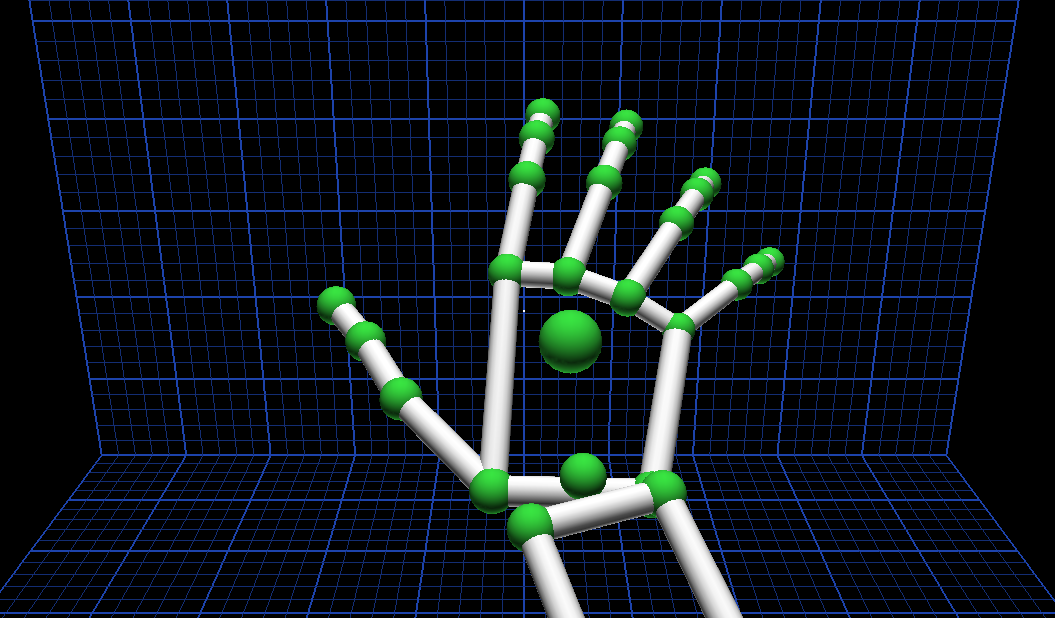
\includegraphics[width=7cm]{images/SDK_LeapMotion.png}
    \end{figure}
  \item RealSense est un périphérique relativement récent à mis chemin entre Kinect 2 et LeapMotion. On peut, à l'aide du SDK fournis, récupérer des informations semblables à celles fournies par LeapMotion : 
  22 points de la main détectés et suivits
\end{itemize}
\ \\
Les données en RGB peuvent être utiliser avec des accessoires colorés pour simplifier la détection des points de la main. \cite{wang2009real} 
Elles peuvent également être associées avec des données de profondeur pour améliorer la détection et gérer les cas de superposition. \cite{van2011combining}

\section{Modélisation de la main}
%input
Pour mieux visualiser les actions réalisées par la main de l'utilisateur, il est nécessaire d'avoir
un modèle de la main qui soit réaliste et précis par rapport à la réalité. Pour cela, nous avons besoin d'un
mesh d'une main modèle que nous allons ensuite adapté à la main de l'utilisateur.\\

%icp
La méthode utilisé par \cite{export:217428} permet en utilisant l'algorithme
ICP\footnote{Iterated Closest Point} \cite{121791} de modifier le mesh de la main afin
que les points de celui-ci aient une distance moins importante avec le nuage de point fourni pas la 
caméra. Pour cela, l'algorithme ICP recherche les transformations, rotation et translation, qui permettent 
à partir d'un mesh M d'obtenir un mesh P. Dans notre cas, le mesh M représente le modèle de main donné en entré
et le mesh P représente la main de l'utilisateur.\\ 

%squelette TODO trop dur
La méthode de \cite{export:217428} permet également d'adapter le squelette du modèle de la 
main, ce qui permet d'obtenir une précision plus importante lors de l'utilisation de l'application.
Cette méthode se repose sur le calcul de la fonction énergie.

\section{Détection de la main}

La Kinect possède deux types de caméra, une caméra couleur et une caméra de profondeur utilisant la méthode 
\og Time of Flight \fg. Les caméras de type \og Time of Flight \fg envoient des rayons infrarouges. Une caméra infrarouge
récupére ensuite les rayons réfléchit, ce qui permet d'obtenir les informations de profondeur. 
Il existe plusieurs solutions utilisant l'une ou l'autre de ces caméras. Nous allons
dans cette partie détailler plusieurs méthodes réalisées jusqu'à maintenant.

\subsection{Détection et suivi de la main à partir d'une image couleur}
La méthode proposée par S. Bilal et al \cite{haarlike} utilise l'algorithme de Viola et al \cite{viola2001jones} afin
de détecter la main et fournir la position de celle-ci en créant une ROI\footnote{Region Of Interest} autour d'elle.
L'algorithme de Viola et al \cite{viola2001jones} nécessite une 
base de connaissances composée des caractéristiques de l'objet recherché. Elle est utilisée dans un 
apprentissage supervisé, c'est-à-dire que l'algorithme a besoin de données représentant
l'objet à détecter pour classifier les caractéristiques de celui-ci. Cet algorithme est basé sur des caractéristiques 
pseudo-Haar qui crée des masques rectangulaires et adjacents dans différentes zones de l'image (voir Fig. \ref{fig:pseudo_haar}). 
Chaque masque calcule l'intensité des pixels qu'il contient, puis l'algorithme fait la différence entre les masques blancs et 
les masques noirs.\\

\begin{figure}[!h]
\center

\includegraphics[width=7cm]{images/pseudo_haar.png}
\caption{Exemple de caractéristiques pseudo-Haar utilisées pour l'algorithme Viola et Jones}
\label{fig:pseudo_haar}
\end{figure}

Une fois, qu'une ROI est formée autour de la main de l'utilisateur S. Bilal et al \cite{haarlike} changent d'espace colorimétrique
afin de pouvoir différencier la main du reste de l'environnement. Pour cela, S. Bilal et al \cite{haarlike} choisissent 
d'utiliser l'espace YCbCr qui permet d'obtenir des informations de chromaticité dont la valeur est presque équivalente
quelle que soit la couleur de peau de l'utilisateur \cite{yoo1999fast}. Une fois que la ROI de la main est binarisé, il est possible
de détecter le bout des doigts. Il faut tout d'abord calculer le centroïde de la forme de la main, puis la distance entre
ce centroïde et chaque point du contour de la main. Le coutour d'une forme dans une image est défini par un changement brutal
de couleur. Cette méthode permet d'obtenir un graphe correspondant à la Fig. \ref{fig:handHisto}, où chaque pique représente un doigt.

\begin{figure}[!h]
\center
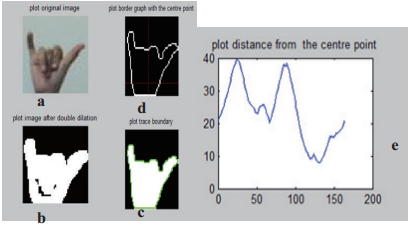
\includegraphics[width=7cm]{images/handHisto.png}
\caption{Histogramme des distances entre les points du contour de la main et le centroide}
\label{fig:handHisto}
\end{figure}

Afin de pouvoir traquer la main, S. Bilal et al \cite{haarlike} utilisent l'algorithme de Kalman \cite{kalman}.
Cet algorithme permet de prédire la position d'un objet, ainsi dans la méthode que nous étudions la main sera traquée malgrès
le bruit présent dans l'image. De plus, cette méthode n'a besoin de connaître que l'état précédent à celui 
qui est calculé.

\subsection{Détection et suivi de la main avec une image de profondeur}
Une seconde solution utilise une image de profondeur plutôt que l'image binarisée grâce au changement d'espace colorimétrique.
Pour réaliser la détection de la main, il faut dans un premier temps déterminer une ROI
autour ce celle-ci. Cette première étape a été expliqué par T. Sharp et al\cite{export:238453}, où les auteurs utilisent un classifieur
qui se repose sur la méthode développée dans \cite{export:145347}. Ce classifieur permet d'effectuer de la reconnaissance
des parties du corps et permet également de détecter les articulations.
%TODO essayer d'expliquer mieu le fonctionnement de kinect
\begin{figure}[!h]
 \begin{center}
  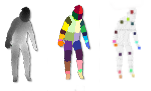
\includegraphics[width=7cm]{images/bodyrecognition.png}
  \caption{Résultat de la détection des parties du corps et des articulations grâce à la méthode de \cite{export:145347}}
  \label{fig:bodyrecognition}
 \end{center}
\end{figure}

\newpage

On voit sur la Fig. \ref{fig:bodyrecognition} que l'articulation de la main est détecté, il est alors possible de construire
une ROI autour de ce point. Cette méthode a été implémenté dans la caméra Kinect.\\

La méthode utilisé dans \cite{export:238453} ne nécessite aucune donnée provenant d'image antérieur. L'ensemble
des calculs sont réalisés sur une image à partir d'une base de connaissance contenant différente posture de la
main. Etant donnée qu'il est impossible de stocker toutes les postures de la main, la méthode de \cite{export:238453}
calcule une fonction energy permettant de déterminer quel est la posture la plus représentative de celle de la main
de l'utilisateur. Cette fonction energy est calculé à partir des pixels du modèle et ceux de l'image de profondeur
capturé par la caméra. Elle est défini par le calcul suivant :
\begin{equation}
 E^{au}(Z_{roi}, R_{roi}) = \sum_{ij} \bar{\rho(z_{ij}} - r_{ij})
\end{equation}
Dans cette équation, $z_{ij}$ représente la pixel à la position (i,j) dans le modèle et $r_{ij}$ représente le pixel à la position (i,j)
provenant de l'image de profondeur. La fonction $\rho(e)$ quand à elle est équivalent à $min(|e|,\tau)$ ou $\tau$ est une valeur fixe permettant
d'éliminer le bruit présent dans l'image de profondeur.

\section{Evaluation des solutions envisagées}
